\documentclass[12pt]{article}

\title{Real dimension in the Newtonian simulation of disk-like pressure-free systems}
\author{S. Halayka\footnote{sjhalayka@gmail.com}}
\date{\today\;\currenttime}

\usepackage{datetime}
\usepackage{listings}
\usepackage{cite}
\usepackage{xcolor}
\usepackage{graphicx}
\usepackage{setspace}
\usepackage{amsmath}
\usepackage{url}
\usepackage[margin=0.8in]{geometry}
\usepackage{listings}


\usepackage{xcolor}
\lstset { %
    language=C++,
    backgroundcolor=\color{black!5}, % set backgroundcolor
    basicstyle=\footnotesize,% basic font setting
    showstringspaces=false,
}


%\doublespace

%\usepackage[]{lineno}
%\linenumbers


\begin{document}



 
\maketitle

\begin{abstract}
This paper contains a short introduction to Newtonian gravitation.
The main focus is on some C++ code.
\end{abstract}






\section{Brute force: field line intersection density gradient}
Regarding the holographic principle, where $n$ is the gravitational field line count, and $A_s$ is the Schwarzschild black hole event horizon area:
\begin{equation}
n = \frac{A_s k c^3}{ 4 G \hbar \log 2},
\end{equation}
the Schwarzschild radius is:
\begin{equation}
r_s = \sqrt{\frac{A_s}{4 \pi}} = \sqrt{\frac{n G \hbar \log 2}{k c^3 \pi}},
\end{equation}
and the mass is:
\begin{equation}
M = \frac{c^2 r_s}{2 G} = \sqrt{\frac{n c \hbar \log 2}{4 G k \pi}}. 
\end{equation}

Where $R$ is some far distance from the centre of the gravitating body (e.g, $R \gg r_s$), $\beta$ is the get intersecting line length function, and $\epsilon$ is some small value (e.g $10^{-5}$), the gradient is:
\begin{equation}
\gamma = \frac{\beta(R + \epsilon) - \beta(R)}{\epsilon}.
\end{equation}
The gradient strength is:
\begin{equation}
g = -\gamma \pi = \frac{n}{2 R^3}.
\end{equation}
From this we can get the Newtonian acceleration $a$ for a flat rotation curve of speed $v$:
\begin{equation}
\label{a_equation}
a = \frac{v^2}{R} = \frac{g R c \hbar \log 2}{k 2 \pi M},
\end{equation}
\begin{equation}
v = \sqrt{\frac{g R^2 c \hbar \log 2}{k 2 \pi M}}.
\end{equation}


\begin{figure} 
\centering
\label{fig1}
  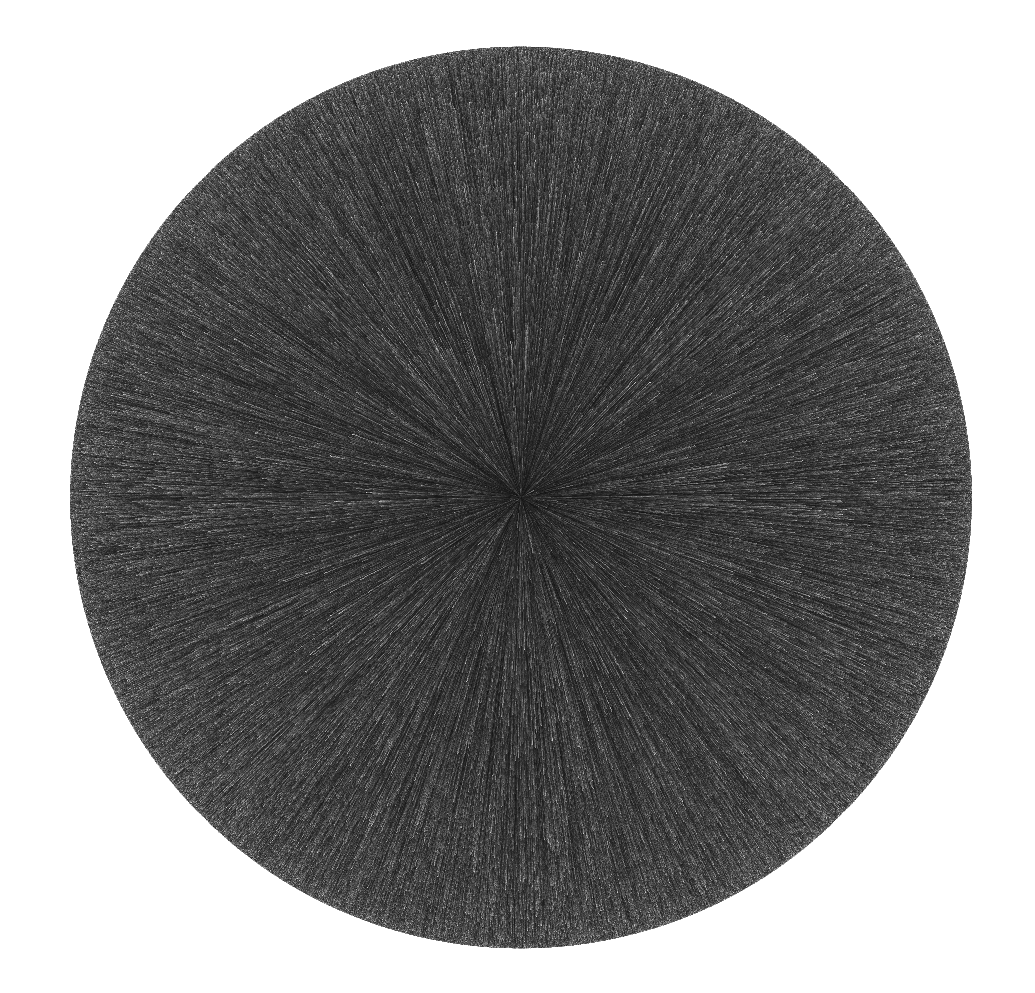
\includegraphics[width = 4 in]{3.png}
  \caption{
Where $D = 3$.
}
\end{figure}

\begin{figure} 
\centering
\label{fig2}
  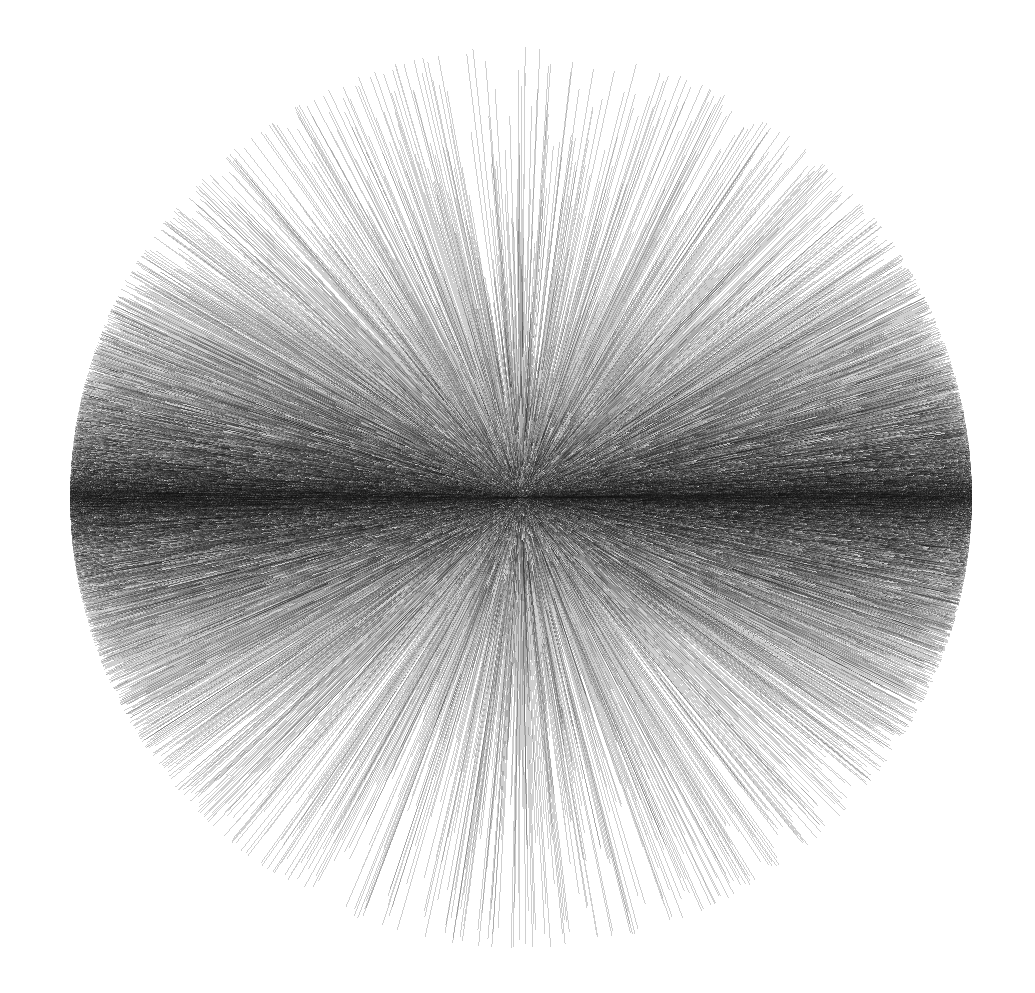
\includegraphics[width = 4 in]{2.1.png}
  \caption{
Where $D = 2.1$.
}
\end{figure}




\section{Heuristic: field line intersection density gradient}

For example, where $D = 2.001$, the ratio of the acceleration is
\begin{equation}
\frac{a_{D}}{a_{3}} = R^{d}, 
\end{equation}
where $d = 3 - D = 0.999$.
Here $d$ stands for disk-like.

The code for this section can be downloaded from:

\url{https://github.com/sjhalayka/ellipsoid_emitter}





%\pagebreak







\begin{thebibliography}{9}

\bibitem{misner} Misner et al. Gravitation. (1970)

\bibitem{hooft} `t Hooft. Dimensional reduction in quantum gravity. (1993)
\bibitem{susskind} Susskind. The World as a Hologram. (1994)





%\bibitem{nasa} Williams. NASA Mercury Fact Sheet. (2024)



\end{thebibliography}














\end{document}









